\documentclass{beamer}

\usetheme{CambridgeUS}
\usepackage{graphicx}
\usepackage{hyperref}

\title{Social Algorithms and Optimization}
\author{Jorge Aldair Cortés López}
\institute{Centro de Investigación en Computación}
\date{\today}

\begin{document}

\begin{frame}
    \titlepage
\end{frame}

\begin{frame}{Contenido}
    \tableofcontents
\end{frame}

\section{Referencias}

\begin{frame}{Referencias}
\begin{thebibliography}{30}
\bibitem{faridmehr2023mtbo}
I. Faridmehr, M.L. Nehdi, and I.F. Davoudkhani,
"Mountaineering team-based optimization: A novel human-based metaheuristic algorithm",
\textit{Mathematics}, vol. 11, no. 5, 2023.
Available at: \url{https://www.mdpi.com/2227-7390/11/5/1273}.

\bibitem{srinivasan2013social}
S. Srinivasan and S. Ramakrishnan,
"A social intelligent system for multi-objective optimization of classification rules using cultural algorithms",
\textit{Computing}, vol. 95, no. 1, pp. 21–45, 2013. 
Available at: \url{https://link.springer.com/article/10.1007/s00607-012-0246-4}.

\bibitem{6973911}Gong, Y., Zhang, J. \& Li, Y. From the social learning theory to a social learning algorithm for global optimization. {\em 2014 IEEE International Conference On Systems, Man, And Cybernetics (SMC)}. pp. 222-227 (2014)

\end{thebibliography}
\end{frame}

\begin{frame}{Referencias}
\begin{thebibliography}{30}
\bibitem{altay2019performance}
E.V. Altay and B. Alatas,
"Performance comparisons of socially inspired metaheuristic algorithms on unconstrained global optimization",
\textit{Proceedings of IC4S}, Springer, 2019. 
Available at: \url{https://link.springer.com/chapter/10.1007/978-981-13-0341-8_15}.

\bibitem{kulkarni2018socio}
M. Kumar, A.J. Kulkarni, and S.C. Satapathy,
"Socio evolution \& learning optimization algorithm: A socio-inspired optimization methodology",
\textit{Future Generation Computer Systems}, vol. 88, pp. 653–674, 2018.
Available at: \url{https://www.sciencedirect.com/science/article/pii/S0167739X17317259}.

\bibitem{maheri2021survey}
A. Maheri, S. Jalili, Y. Hosseinzadeh, and R. Khani,
"A comprehensive survey on cultural algorithms",
\textit{Swarm and Evolutionary Computation}, 2021. 
Available at: \url{https://www.sciencedirect.com/science/article/pii/S2210650221000079}.

\end{thebibliography}
\end{frame}


\begin{frame}{Referencias}
\begin{thebibliography}{30}

\bibitem{kumar2019socio}
M. Kumar and A.J. Kulkarni,
"Socio-inspired optimization metaheuristics: A review",
in \textit{Socio-cultural inspired metaheuristics}, Springer, 2019.
Available at: \url{https://link.springer.com/chapter/10.1007/978-981-13-6569-0_12}.

\bibitem{jalili2022cultural}
S. Jalili,
"Cultural Algorithms",
in \textit{Engineering Optimization: Methods and Applications}, Springer, 2022.
Available at: \url{https://link.springer.com/content/pdf/10.1007/978-981-19-4633-2.pdf}.

\bibitem{Neme2009}Neme, A. \& Hernández, S. Algorithms Inspired in Social Phenomena. {\em Nature-Inspired Algorithms For Optimisation}. pp. 369-387 (2009),  \url{https://doi.org/10.1007/978-3-642-00267-0_13}

\end{thebibliography}
\end{frame}


\section{Contenido}
\begin{frame}{Antecedentes}
    \begin{itemize}
        \item La evolución de los algoritmos bioinspirados (Nature-inspired algorithms) se corresponde con la evolución de los sistemas naturales.         
    \end{itemize}

    \vspace{0.5cm}
    \centering
    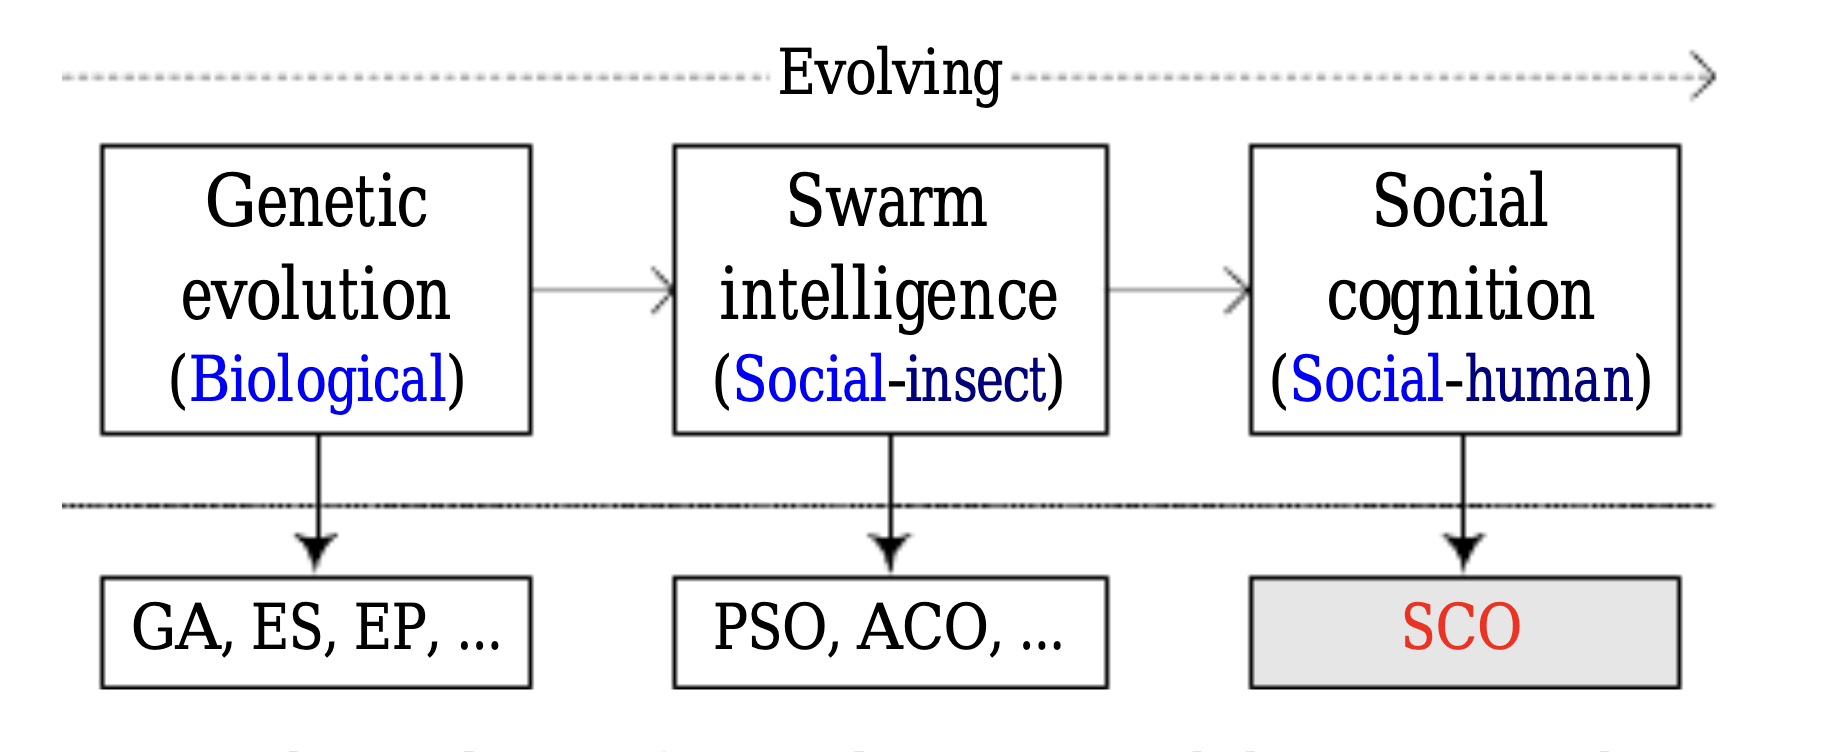
\includegraphics[width=0.9\textwidth]{classification_1.png}

\end{frame}

\begin{frame}{Antecedentes}
    \begin{itemize}
        \item Se propone en la literatura, la siguiente clasificación de los algoritmos bioinspirados  
    \end{itemize}

    \vspace{0.5cm}
    \centering
    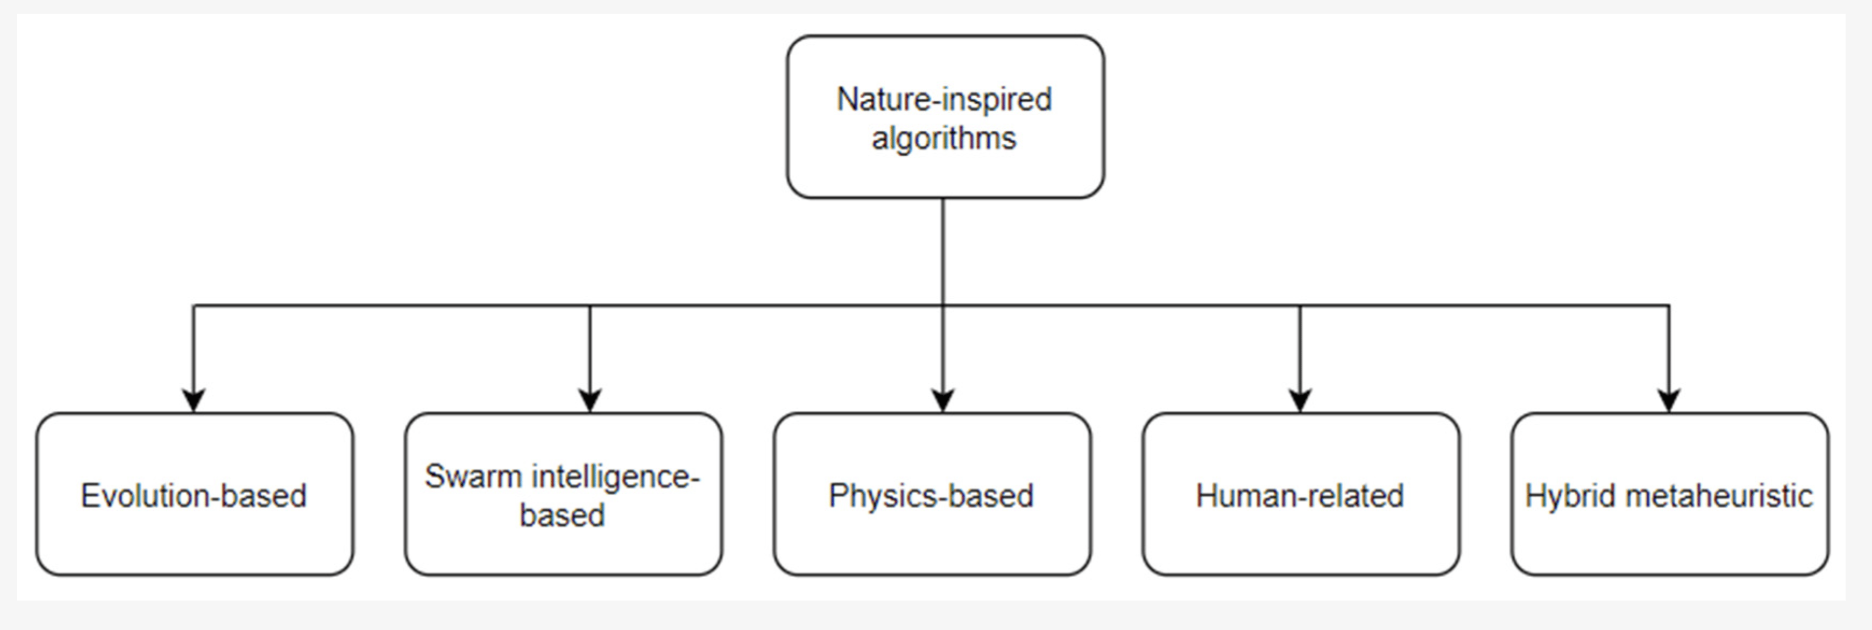
\includegraphics[width=0.9\textwidth]{classification_2.png}

\end{frame}

\section{Modelo basado en traducción}

\begin{frame}{Modelo basado en traducción}
    \begin{itemize}
        \item Las relaciones $(h, \ell, t)$ son modeladas como $h + \ell \approx t$.
        \item Utiliza una función de disimilitud ($L_1$ o $L_2$) para calcular energías:
        \[
        d(h + \ell, t)
        \]
        \item Entrenamiento:
        \begin{itemize}
            \item Minimizando una función de pérdida basada en márgenes.
            \item Algoritmo de gradiente estocástico.
        \end{itemize}
        \item Embeddings con restricciones normativas para evitar sobreajuste.
    \end{itemize}
    \vspace{0.5cm}
    \centering
    \includegraphics[width=0.6\textwidth]{placeholder_image} % Espacio para ecuaciones o diagramas
\end{frame}


\section{Trabajos relacionados}

\begin{frame}{Trabajos relacionados}
    \begin{itemize}
        \item Comparación con otros modelos:
        \begin{itemize}
            \item Structured Embeddings (SE).
            \item Neural Tensor Model (NTM).
        \end{itemize}
        \item \textbf{Ventaja encontrada:} TransE es más simple y eficiente, evitando problemas de optimización complejos.
        \item Se menciona en el artículo sobre la comparación con SE: \textit{ Despite the lower expressiveness of our model, we still reach better performance than
SE in our experiments. We believe this is because: \\
\begin{enumerate}
    \item Our model is a more direct way to represent the true properties of the relationship,
    \item optimization is difficult in embedding models.
\end{enumerate}}
    \end{itemize}
    \vspace{0.5cm}
    \centering
    \includegraphics[width=0.6\textwidth]{placeholder_image} % Espacio para un gráfico comparativo
\end{frame}

\begin{frame}{Ecuación de perdida}
\begin{center}
        \includegraphics[width=0.9\textwidth]{table2.png} % Espa
\end{center}
\end{frame}

\section{Experimentos}

\subsection{Conjuntos de datos y configuración}

\begin{frame}{Conjuntos de datos y configuración}
    \begin{itemize}
        \item Bases utilizadas:
        \begin{itemize}
            \item WordNet.
            \item Freebase (FB15k y FB1M).
        \end{itemize}
        \item Métricas:
        \begin{itemize}
            \item Mean Rank.
            \item Hits@10.
        \end{itemize}
    \end{itemize}
    \vspace{0.5cm}
    \centering
    \includegraphics[width=0.9\textwidth]{table1.png} % Espacio para una tabla de datos
\end{frame}

\subsection{Resultados y conclusiones experimentales}

\begin{frame}{Resultados y conclusiones experimentales}
    \begin{itemize}
        \item TransE supera a otros métodos en la mayoría de las métricas y escenarios.
        \item Ejemplo: Hits@10
        \begin{itemize}
            \item WordNet: 89.2\%.
            \item Freebase FB15k: 47.1\%.
        \end{itemize}
        \item Limitaciones:
        \begin{itemize}
            \item Menor eficacia en relaciones ternarias complejas.
        \end{itemize}
    \end{itemize}
    \vspace{0.5cm}
    \centering
    \includegraphics[width=0.9\textwidth]{table3.png} % Es
\end{frame}
\begin{frame}{Ejemplo de predicción}
    \vspace{0.5cm}
    \centering
    \includegraphics[width=0.9\textwidth]{table5.png} % Espacio para un gráfico de resultados
\end{frame}
\section{Conclusión y trabajo futuro}

\begin{frame}{Conclusión y trabajo futuro}
    \begin{itemize}
        \item \textbf{Conclusiones:}
        \begin{itemize}
            \item TransE es un modelo simple y escalable.
            \item Exitoso en la predicción de enlaces en grandes bases de conocimiento.
        \end{itemize}
        \item \textbf{Trabajo futuro:}
        \begin{itemize}
            \item Extender el modelo a dominios con relaciones más complejas.
            \item Combinar embeddings con datos textuales.
        \end{itemize}
    \end{itemize}
    \vspace{0.5cm}
    \centering
    \includegraphics[width=0.9\textwidth]{table6.png} % E
\end{frame}

\end{document}